\documentclass[../main.tex]{subfiles}

\begin{document}

The core part of the implementation of any asynchronous task within Reqour is \textbf{asynchronous task executor}, whose design is depicted in Figure \ref{fig:task-executor}. Its implementation uses \textit{CompletableFuture}\footnote{\url{https://docs.oracle.com/en/java/javase/21/docs/api/java.base/java/util/concurrent/CompletableFuture.html}} API in order to execute the task asynchronously.

The implementation is shown in Listing \ref{lst:task-executor}\footnote{\url{https://github.com/project-ncl/reqour/blob/akridl-thesis/core/src/main/java/org/jboss/pnc/reqour/common/executor/task/TaskExecutorImpl.java##L36-L45}}. At line 7, we are using managed executor\footnote{\url{https://download.eclipse.org/microprofile/microprofile-context-propagation-1.0/apidocs/org/eclipse/microprofile/context/ManagedExecutor.html}} which invokes synchronous function on an underlying thread, hence, not blocking caller thread. At line 8, in case of an exception, we handle it appropriately. Finally, at line 9, the callback is being sent using the provided callback sender.

\begin{lstlisting}[language=Java, caption=Asynchronous task executor, label={lst:task-executor}]
public <T, R> void executeAsync(
        Request callbackRequest,
        T request,
        Function<T, R> syncExecutor,
        BiFunction<T, Throwable, R> errorHandler,
        BiConsumer<Request, R> callbackSender) {
    executor.supplyAsync(() -> syncExecutor.apply(request))
            .exceptionally(t -> errorHandler.apply(request, t))
            .thenAccept(res -> callbackSender.accept(callbackRequest, res));
}
\end{lstlisting}

\begin{figure}
  \begin{center}
    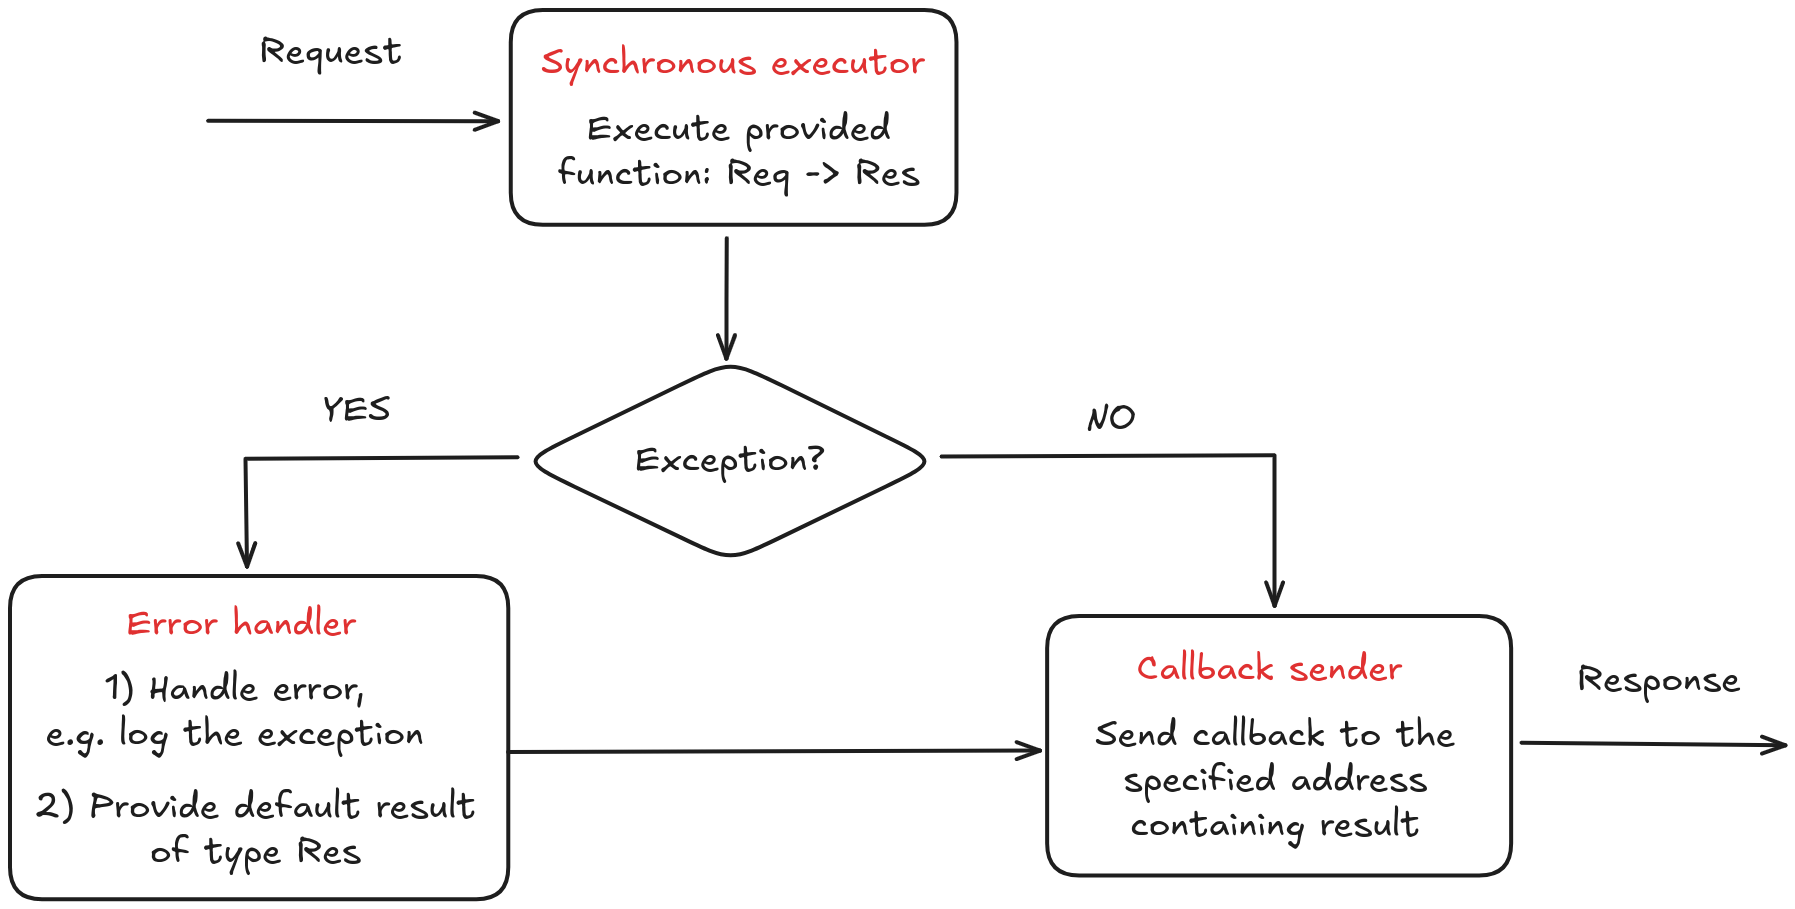
\includegraphics[width=\textwidth]{images/task-executor.png}
  \end{center}
  \caption{High-level overview of asynchronous task executor}
  \label{fig:task-executor}
\end{figure}

The implementation of internal SCM repository creation itself contains just call to asynchronous task executor, see Listing \ref{lst:internal-scm-handler}\footnote{\url{https://github.com/project-ncl/reqour/blob/akridl-thesis/rest/src/main/java/org/jboss/pnc/reqour/rest/endpoints/InternalSCMRepositoryCreationEndpointImpl.java##L50-L59}}.

\begin{lstlisting}[language=Java, caption=Internal SCM repository creation endpoint handler, label={lst:internal-scm-handler}]
public void createInternalSCMRepository(InternalSCMCreationRequest creationRequest) {
    taskExecutor.executeAsync(
            creationRequest.getCallback(),
            creationRequest,
            service::createInternalSCMRepository,
            this::handleError,
            callbackSender::sendInternalSCMRepositoryCreationCallback);

    throw new WebApplicationException(Response.Status.ACCEPTED);
}
\end{lstlisting}

\subsubsection*{Attached PRs}
\subfile{./subsubsections/prs}

\end{document}
